\documentclass{hcmutarticle}

% gói để tạo chữ giả, xóa đi khi viết báo cáo
\usepackage{lipsum}

% create the header for this file
\fancyhead[RO, LE]{\bf Bài toán khai báo tài liệu trích dẫn}


\begin{document}
\thispagestyle{empty}
\begin{center}
\LARGE\bfseries ĐẠI HỌC QUỐC GIA TP HỒ CHÍ MINH \\
TRƯỜNG ĐẠI HỌC BÁCH KHOA
\end{center}

\begin{center}

\includegraphics[scale=0.2]{hcmut.pdf}\\[1cm]
\end{center}

\vspace{1cm}

\begin{center}
\Large \bfseries HƯỚNG DẪN KHAI BÁO TÀI LIỆU TRÍCH DẪN THEO CÁC  CHUẨN SẴN CÓ \\[0.5cm]
\end{center}
\rule{\textwidth}{1pt}
\vspace{2pt}
\begin{center}
\Huge
\begin{tabular}{@{}l}
Bài toán khai báo tài liệu trích dẫn\\[6pt]
\end{tabular}
\end{center}
\rule{\textwidth}{1pt}\\[1cm]

\vspace{3cm}

\begin{minipage}[t]{0.60\linewidth}
\textbf{GVHD}: \\
\ Nguyễn Thanh Hùng
\end{minipage}
\begin{minipage}[t]{0.40\linewidth}
\textbf{Sinh viên thực hiện:}\\
Nguyễn Quốc Long - MSSV:51101909\\
Đinh Tấn Lộc - MSSV:51101935
\\Nguyễn Sang Trường Sơn-MSSV:51102938
\\Huỳnh Tấn Ngàn-MSSV:51102184
\end{minipage}

\vspace{3cm}

\begin{center}

\textbf{TP.Hồ Chí Minh},
20/05/2012.

\end{center}



\newpage

\tableofcontents 

\newpage

\title{Bài toán khai báo tài liệu trích dẫn}

\author{  Nguyễn Quốc Long\inst{1} 
\and Đinh Tấn Lộc\inst{2}
\and Nguyễn Sang Trường Sơn \inst{3}
\and Huỳnh Tấn Ngàn \inst{4}}
\institute{ MSSV: 51101909
\and  MSSV: 51101935
\and  MSSV: 51102938
\and  MSSV: 51102184}



\maketitle



\begin{abstract}
Tài liệu nêu ra các chuẩn trình bày các tài liệu tham khảo, 


\end{abstract}

\begin{keywords}
Tài liệu trích dẫn, khai báo tài liệu trích dẫn, trình bày trích dẫn..
\end{keywords} 


\section{Giới thiệu}

\textbf{Một văn bản} 
 bao giờ cũng có một số tài liệu tham khảo, nhất là một luận án tốt nghiệp hay luận án tiến sỹ thì làm danh sách tài liệu tham khảo cực kỳ quan trong. Một cuốn sách in ra phải có phần tham khảo các tài liệu khác, rất nhiều viết sách rõ ràng là chép của người khác mà không thấy liệt kê các sách tham khảo.


Trong quá trình học tập, nghiên cứu, khi viết báo cáo chúng ta thường xuyên phải tham khảo tài liệu bên ngoài có liên quan, vì vậy việc trích dẫn những tài liều mà mình đã tham khảo là cần thiết và không thể tránh khỏi.\\
\textbf{Bạn đã từng..?} .\\
$-$   Mua hoặc có được toàn bộ bài viết/ công trình nghiên cứu của người khác và nhận đó là công trình của mình ?\\
$- $  Sử dụng thông tin hoặc ý tưởng cụ thể từ một nguồn bên ngoài, trích dẫn tài liệu nhưng không diễn giải bằng từ ngữ của chính mình?\\
$- $  Sao chép nguyên các đoạn, câu hoặc cụm từ dài từ bách khoa toàn thư hoặc các nguồn thông tin trên mạng khác, sau đó chèn các phần này vào bài viết của mình mà không trích dẫn?\\
$- $  Sao chép các đoạn văn bản từ bài viết của người khác?\\
$- $  Dùng thông tin chi tiết từ sách giáo khoa hoặc một nguồn khác làm tài liệu nền cho bải viết của mình mà không trích nguồn?\\
$- $  Sử dụng cấu trúc bài viết, ý tưởng hoặc từ ngữ của người khác. Tác giả của các tài liệu đó nếu cho phép sao chép thì cũng bị xem là đạo văn?\\


 Trong tài liệu này chúng sẽ giới thiệu cho các bạn cách trích dẫn tài liệu tham khảo theo các chuẩn có sẵn trong Latex. Hy vọng tài liệu sẽ thực sự hữu ích cho các bạn.\\

\newpage

%%%%%%%%%%%%%%
\section{Tóm tắt nội dung}\label{survey}
Một văn bản bao giờ cũng có một số tài liệu tham khảo, nhất là một luận án tốt nghiệp hay luận án tiến sỹ thì làm danh sách tài liệu tham khảo cực kỳ quan trong. Một cuốn sách in ra phải có phần tham khảo các tài liệu khác, rất nhiều viết sách rõ ràng là chép của người khác mà không thấy liệt kê các sách tham khảo.\\
{\bfseries  Sau đây là cách trích dẫn tài liệu tham khảo theo quy định của Bộ Giáo Dục và Đào Tạo:}\\

Trong bài viết, bất cứ dẫn chứng nào cũng phải kèm tên tác giả và thời điểm công bố (xuất bản). Nếu tác giả người nước ngoài chỉ cần liệt kê HỌ. Nếu tài liệu chuyển ngữ sang tiếng Việt , cách dẫn chứng như trên.Nếu tác giả là người Việt hoặc tiếng nước ngoài thì liệu kê đầy đủ như chính tác giả đã viết.\\
Sau đây, chúng ta sẽ đi vào cụ thể từng chuẩn khai báo tài liệu trích dẫn.
%%%%%%%%%%%%%%
\section{Giới thiệu vấn đề }\label{dev}
Các phương pháp trích dẫn

\subsection{Phong cách ACS (ACS Style Guide)}

Phong cách ACS là một tập hợp các tiêu chuẩn cho các văn bản tài liệu liên quan đến hóa học, bao gồm cả một phương pháp tiêu chuẩn của trích dẫn trong ấn phẩm học thuật , phát triển bởi Hiệp hội Hóa học Mỹ (ACS). Các phiên bản in của các hướng dẫn phong cách ACS: truyền thông hiệu quả thông tin khoa học , lần thứ 3. (2006), thay đổi nội dung bởi Coghill Anne M. và Garson Lorrin R.

\subsubsection{Làm thế nào để định dạng văn bản trích dẫn}.

Chọn một trong ba phương pháp dưới đây để trích dẫn trong văn bản tài liệu tham khảo:

\paragraph{Superscript số}.

{\em Vào cuối của các thông tin được trích dẫn:}

fluoride nước cũng như các sản phẩm có chứa chất florua khác nhau như kem đánh răng cung cấp các ion florua cần thiết cho remineralization 1.

{\em Trong các thông tin được trích dẫn:}

Rakita 1 nói rằng nước có chất fluoride cũng như các sản phẩm có chứa chất florua khác nhau như kem đánh răng cung cấp các ion florua cần thiết cho remineralization.


\paragraph{Nghiêng số}.

{\em Vào cuối của các thông tin được trích dẫn:}

fluoride nước cũng như các sản phẩm có chứa chất florua khác nhau như kem đánh răng cung cấp các ion florua cần thiết cho remineralization ( {\itshape 1} ).

{\em Trong các thông tin trích dẫn:}

Rakita ( {\itshape 1} ) tuyên bố rằng nước có chất fluoride cũng như các sản phẩm có chứa chất florua khác nhau như kem đánh răng cung cấp các ion florua cần thiết cho remineralization.


\paragraph{Tên tác giả và năm xuất bản}.

{\em Vào cuối của các thông tin được trích dẫn:}

fluoride nước cũng như các sản phẩm có chứa chất florua khác nhau như kem đánh răng cung cấp các ion florua cần thiết cho remineralization (Rakita, 2004).

{\em Trong các thông tin trích dẫn:}

Rakita nước có chất fluoride cũng như các sản phẩm có chứa chất florua khác nhau như kem đánh răng cung cấp các ion florua cần thiết cho remineralization (2004).

\paragraph{Làm thế nào để định dạng danh sách tham khảo}.

{\bfseries Sách}

{\em Độc thân tác giả}

Chang, R. Tổng Hóa: Các khái niệm cần thiết, lần thứ 3, McGraw-Hill: Boston, năm 2003.

{\em Thay đổi nội dung sách}

Gbalint-Kurti, GG Wavepacket Lý thuyết của hình ảnh phân li và tán xạ phản ứng. 
{\em Sách trong Series}

Omega-3 axit béo: Hóa học, dinh dưỡng, Y tế và ảnh hưởng; Shahidi, F., Finley, JW, Eds; ACS Hội thảo Series 788; Hội Hóa học Mỹ: Washington, DC năm 2001.

{\em Điều từ một cuốn sách tham khảo}

Luyện kim bột. Kirk-Othmer Bách khoa toàn thư của Công nghệ hóa học, lần thứ 3; Wiley: New York, năm 1982, Vol. 19, Trang 28-62.

{\bfseries Các bài viết}

{\em Bài báo trong một tạp chí khoa học}

Evans, DA; Fitch, DM, Smith, TE; Cee, VJ Áp dụng các phản ứng nghịch đảo phức tạp để tổng hợp Phorboxazole B. J. Am. Chem. Sóc 2000, 122 , 10033-10046.

{\em Bài báo trong một tạp chí phổ biến / không khoa học}

Manning, R. Siêu hữu cơ, 2004, pp 176-181.

{\em Điều từ một tạp chí trực tuyến}

Peacock-Lopez, E. Chính xác giải pháp tiềm năng Quantum. 2007, 11 , 383-393 http://chemeducator.org/bibs/0011006/11060380lb.htm 

{\bfseries Luận án, Bằng sáng chế, Hội nghị, Báo cáo kỹ thuật}

{\em Đề tài}

Thoman, JW, Jr nghiên cứu của vô hiệu hóa một phân tử hoạt động bề mặt -Tiến sĩ Luận án, Viện Công nghệ Massachusetts, Cambridge, MA, 1987.
hoăc

Gehring, A. Tiến sĩ. Luận văn, Đại học Harvard năm 1998.

{\em Bằng sáng chế}

 Phát hiện, cách ly, Thanh lọc độc tố Clostridiu, ngày 24 tháng 3 1992.

{\em Hội nghị / Hội nghị (toàn văn)}

Winstein, Trong Giáo dục Đại học Hóa chất, Kỷ yếu của Hội nghị Quốc tế về Giáo dục Đại học Hóa chất, Frascati (Rome), Italy, 16-19 tháng Mười, năm 1969; Chisman, DG. Ed; Butterworths: London, 1970.

{\em Hội nghị / cuộc họp }

Kaplan, LJ; Selder, A. sách tóm tắt, 213th ACS Hội nghị Quốc gia, San Francisco, CA, 13-ngày 17 tháng tư, năm 1997, Hội Hóa học Mỹ: Washington, DC, năm 1997, CHED-824.

{\em Báo cáo kỹ thuật }

Crampton, SB; McAllaster, hiệu ứng chuyển động trung bình trong maser nguyên tử Hydrogen đông lạnh, WMC-AFOSR-002; NTIS: Springfield, VA, 1983.

{\bfseries Web / Mạng}

Lưu ý: trình duyệt web khác nhau phá vỡ các văn bản ở những nơi khác nhau của một URL. URL nên bắt đầu trên cùng một dòng như phần còn lại của các thông tin trích dẫn, với một đoạn chèn vào sau khi một dấu gạch chéo, nếu cần thiết.

{\em Trang web}

National Library of Medicine. Y tế và môi trường Độc Chất: Dịch vụ Thông tin chuyên ngành. http://sis.nlm.nih.gov/enviro.html (truy cập ngày 23 tháng 8 2004.

{\em Điều từ một tạp chí trực tuyến}

Peacock-Lopez, E. Chính xác Giải pháp tiềm năng Quantum. Chem. Ed. 2007, 11 , 383-393 http://chemeducator.org/bibs/0011006/11060380lb.htm (truy cập ngày 23 tháng 8 năm 2007).

{\em Điều từ cơ sở dữ liệu văn bản đầy đủ}

Begley, S. Khi não của bạn ngừng hoạt động Newsweek [Online] ngày 02 Tháng Bảy 2007, 62 p. Mở rộng. http:/galegroup.com (truy cập ngày 23 tháng 8 năm 2007).



\subsection{Phong cách dành cho tác giả và biên tập viên (AMA manual of style)}

{\em AMA Manual of Style}: Hướng dẫn dành cho Tác giả và biên tập viên là một hướng dẫn phong cách bởi các biên tập viên của JAMA (Tạp chí của Hiệp hội Y khoa Mỹ) và tạp chí - gần đây nhất xuất bản Oxford University Press [ 1 ] [ 2 ] . Quy định cụ thể bằng văn bản và trích dẫn phong cách cho sử dụng trong các ấn phẩm học thuật trong y học quốc tế, bao gồm cả JAMA và tạp chí - . Nó được xuất bản lần đầu vào năm 1962, và phiên bản hiện tại của nó, 10, ra đến năm 2007 [ 1 ] . Hướng dẫn AMA của phong cách bao gồm một bề rộng chủ đề cho tác giả và biên tập viên trong y học và các lĩnh vực liên quan đến sức khỏe và bao gồm 25 chương:{\em Phần 1. Chuẩn bị Điều Xuất bản - 1 loại điều, 2 Chuẩn bị bản thảo, 3 Tham khảo 4 Visual trình bày dữ liệu, 5 Xem xét đạo đức và pháp lý, 6 biên tập đánh giá và chế biến; Mục 2. (US) - 7. Ngữ pháp, 8. Dấu chấm câu, 9. Số nhiều, 10. Hoa, 11. Chính xác và ưu tiên sử dụng, 12. Không phải tiếng Anh từ, cụm từ, và nhãn hiệu Accent, 13. Chỉ số y tế; Phần 3. Thuật ngữ - 14. Chữ viết tắt, 15. Danh mục này, 16. Eponyms, 17. Hy Lạp Thư Mục 4. Đo lường và định lượng 18. Các đơn vị đo lường, 19. Số và Tỷ lệ phần trăm, 20.Thiết kế nghiên cứu và thống kê, 21. Thành phần toán học; Mục 5. Thông tin kỹ thuật - 22. Kiểu chữ, 23. Chỉnh sửa bản thảo và Soát lỗi, 24.Glossary Số Publishing, 25. Tài nguyên.}
\subsubsection{Danh sách tham khảo}.

Tham khảo thông tin sử dụng được thực hiện trong danh sách tham khảo. Điều này bao gồm nhưng không phải là giới hạn các bài báo được công bố hoặc được chấp nhận cho công bố trong in ấn hàng loạt nghiên cứu hoặc lưu thông hoặc tạp chí điện tử, tạp chí, báo, cuốn sách đã được công bố, chấp nhận cho xuất bản, giấy tờ trình bày tại các cuộc họp chuyên nghiệp, tóm tắt, đề tài, CD-ROM, bộ phim, băng hình, và audiofiles, chèn gói hoặc tài liệu hướng dẫn của nhà sản xuất, chuyên khảo; chính thức báo cáo, cơ sở dữ liệu và các trang web, trường hợp pháp luật; bằng sáng chế, và phiên bản mới. Danh sách tham khảo Tài liệu tham khảo cần được liệt kê theo số thứ tự ở phần cuối của bản thảo (trừ trường hợp quy định tại mục 3.3 và 3.5 trong {\itshape Hướng dẫn US AMA}). Hai tài liệu tham khảo không nên kết hợp theo một số tham chiếu duy nhất.

\subsubsection{Tài liệu tham khảo trong văn bản}.


Trích dẫn trong ngoặc trong các văn bản của tài liệu tham khảo đáp ứng các tiêu chuẩn để đưa vào danh sách tài liệu tham khảo nên được giới hạn trường hợp trong danh sách tham khảo sẽ không được sử dụng, tin bài cáo phó. Lưu ý rằng trong các văn bản :

Tài liệu tham khảo trong văn bản Tác giả 

• Có thể không được đặt tên 

• Tiêu đề này có thể không được 

• Tên của tạp chí là viết tắt chỉ khi kèm theo trong ngoặc đơn

 • số trang hòa nhập được 
 
Một số nguồn lực, chẳng hạn như URL Web, có thể được liệt kê trong văn bản khi nó là trang Web chính nó được gọi chứ không phải là nội dung trên trang web đó.

{\bfseries Ví dụ}

Wiese gần đây đã báo cáo rằng chất chiết xuất từ quả của cây xương rồng lê gai có vừa phải có hiệu lực vào việc giảm các triệu chứng nôn nao rượu ({\itshape Arch Intern} Med. 2004; 164 [12] :1334-1340). 

Các tác dụng của chiết xuất từ quả của cây xương rồng lê gai vào việc giảm Các triệu chứng của say rượu cồn đã được báo cáo trong một vấn đề gần đây của tài liệu lưu trữ {\itshape Nội khoa} (2004, 164 [12] :1334-1340). 

{\itshape Archives of Internal Medicine} bài viết (2004, 164 [12] :1334-1340) về tác động của một trích xuất trái cây của cây xương rồng lê gai làm giảm các triệu chứng của rượu nôn nao nhận được công khai rộng rãi (ví dụ, USA Today ngày 29 tháng 6, 2004:7 D)

\subsection{Phong cách báo chí (AP Stypebook)}

{\em AP Stypebook} là một phong cách hướng dẫn sử dụng báo chí và ngành công nghiệp tin tức tại Hoa Kỳ. Các phóng viên, biên tập viên và những người khác sử dụng {\em AP Stylebook} như một hướng dẫn cho dấu chấm câu, ngữ pháp và các nguyên tắc và thực tiễn của báo cáo. Mặc dù một số ấn phẩm sử dụng một hướng dẫn phong cách khác nhau, {\em AP Stylebook} được coi là một tiêu chuẩn ngành công nghiệp báo chí và cũng được sử dụng bởi các đài truyền hình, tạp chí và các công ty quan hệ công chúng. Nó bao gồm một danh sách từ A đến Z hướng dẫn cho viết hoa, viết tắt, chính tả, chữ số và cách sử dụng.
\subsubsection{Chữ số}.

• Sử dụng các số liệu cho các lứa tuổi, số tiền, thời gian trong ngày, tỷ lệ phần trăm, số nhà, năm, ngày tháng, mức độ của nhiệt độ, tỷ lệ, bình chọn, điểm số, tốc độ, thời gian của cuộc đua, kích thước và số serial. 

• Giải thích rõ ràng các con số. Ngoại lệ: Khi bắt đầu một câu với một năm, không viết nó ra. Ví dụ: 1999 là một năm rất tốt. 

• Sử dụng 21 triệu thay vì của 21000000. Ngoài ra: 39 triệu, 22,5 tỷ USD. Không thực hiện vượt quá 2 số thập phân.

• Không sử dụng chữ số La Mã, trừ khi họ là một phần của một tiêu đề hoặc tên. Ví dụ:
Chiến tranh thế giới thứ I, Chiến tranh thế giới thứ II, vua Henry VIII, Rocco Colabella III.

• Chèn dấu chấm với bốn hoặc nhiều hơn con số, ngoại trừ trong ngày. Ví dụ:
5.900, 1.576

\subsubsection{Chữ viết tắt và tiêu đề}.

• Không bao giờ sử dụng một từ viết tắt mà sẽ không được dễ hiểu.

• viết tắt công ty và tập đoàn khi một phần của một tiêu đề của công ty.


\subsubsection{Dấu câu}.

Mục đích của dấu chấm câu là để làm rõ ý nghĩa.

• Đặt dấu chấm vào cuối câu.

• Đặt các trích dẫn vào trong dấu ngoặc kép. Ví dụ:

{\em "Bạn có xem vở kịch?". Ông ta hỏi. 

Tôi có nên xem "King Lear"?}

• Sử dụng dấu gạch ngang để phân biệt ý nghĩa của các từ khác nhau được viết theo cùng một cách. 

• Sử dụng dấu gạch ngang để tách một tiền tố từ một danh từ thích hợp. 

• Khi một trích dẫn nội dung bài viết này một phần được sử dụng, không đặt dấu ngoặc kép quanh trích dẫn đó. 

\subsubsection{Viết hoa}.

• Viết hoa các danh từ riêng và các phần tử phân biệt trong tên của các hiệp hội, xã hội, các công ty, đường phố. Ví dụ: Washington, William Sidney Porter.

• Viết hoa các từ được viết tắt. Ví dụ: WTO, APEC.

\subsection{Phong cách xã hội học Mỹ (The ASA Style Guide)}

{\em Phong cách xã hội học Mỹ }là một định dạng được chấp nhận rộng rãi cho các văn bản tài liệu nghiên cứu trường đại học quy định cụ thể việc bố trí việc sắp xếp và ngắt câu của các ghi chú và thư tịch. Nó được quy định cụ thể trong các {\em hướng dẫn ASA} (US) , được công bố bởi Hiệp hội xã hội học Mỹ , tổ chức nghiên cứu chính cho học tập các nhà xã hội học ở Hoa Kỳ . Hướng dẫn ASA (US) được thiết kế để hỗ trợ các tác giả trong việc chuẩn bị bản thảo cho các tạp chí và ấn phẩm ASA.

\subsubsection{Định dạng bản thảo}.

 • Có một trang tiêu đề riêng biệt cho tên đầy đủ của bài báo, tác giả, vv...
 
 • Nếu cần thiết, trên một trang riêng biệt cung cấp một đoạn ngắn (150 - 200 từ) trừu tượng đứng đầu với tiêu đề của bài báo. 
 
 • Bắt đầu văn bản trên một trang riêng biệt, với tiêu đề của bài báo.
 
 \subsubsection{Trích dẫn trong văn bản}.
 
 • Trực tiếp: Bất cứ khi nào được sử dụng từ chính xác của một tác giả, tài liệu nguồn. 
 o Đối với dấu ngoặc kép: 
 Trích dẫn trong văn bản phải bắt đầu và kết thúc với dấu ngoặc kép, trích dẫn đặt trong dấu trích dẫn và trước thời gian. Ví dụ:
 
 {\em "Năm 1998, tuy nhiên, các dữ liệu được báo cáo theo loại công việc cụ thể cho thấy rằng công việc theo định hướng công nghệ thanh toán tốt hơn " (Hildenbrand 1999:47). 
 
 Hildenbrand báo cáo rằng "vào năm 1998, tuy nhiên, các dữ liệu được báo cáo bởi loại hình làm việc cụ thể hơn cho thấy rằng công việc công nghệ theo định hướng thanh toán tốt hơn "(1999:47). }
 
 
\subsubsection{Danh sách tham khảo}.

• Tất cả các tài liệu tham khảo trích dẫn trong văn bản phải xuất hiện trong danh sách tham khảo. 

• Tất cả các tài liệu tham khảo trong danh sách tham khảo phải được trích dẫn trong văn bản. 

• Sử dụng thụt đầu dòng treo. 

• Giải thích tên tác giả, nếu có hai hoặc nhiều tác giả trong một trích dẫn, để tên tác giả đầu tiên. 

• Danh sách tham khảo nên được sắp xếp theo thứ tự bảng chữ cái tên của tác giả. Nếu là tác giả, sắp xếp các từ quan trọng đầu tiên trong tiêu đề, thứ tự chữ cái trình tự. 

• Sắp xếp nhiều mục của cùng tác giả theo thứ tự năm xuất bản, đầu năm đầu tiên. 

• Phân biệt các công trình của cùng tác giả trong cùng một năm bằng cách thêm chữ, ví dụ như (2003a, 2003b, 2003c). 

• Sử dụng chữ in nghiêng cho cuốn sách và các chức danh định kỳ.


\subsection{Phong cách Chicago (The Chicago Manual of Style) }

{\em The Chicago Manual of Style} (viết tắt trong văn bản như CMS hoặc CMOS, hoặc bằng lời nói như Chicago ) là một hướng dẫn phong cách cho tiếng Anh-Mỹ xuất bản từ năm 1906 bởi Đại học Chicago . Phiên bản 16 đã quy định bằng văn bản và trích dẫn phong cách được sử dụng rộng rãi trong việc xuất bản. Nó là "một trong những hướng dẫn phong cách được sử dụng rộng rãi nhất và tôn trọng tại Hoa Kỳ". Các giao dịch CMS với các khía cạnh thực hành biên tập, từ ngữ pháp tiếng Anh Mỹ và cách sử dụng để chuẩn bị tài liệu.

{\em The Chicago Manual of Style} trình bày hai hệ thống tài liệu cơ bản: (1) ghi chú, thư tịch và (2) chú thích. Lựa chọn giữa hai người thường phụ thuộc vào đối tượng và bản chất của nguồn trích dẫn, như là mỗi hệ thống được ưa chuộng bởi các nhóm khác nhau của các học giả.

Các ghi chú và phong cách thư mục được ưa thích bởi nhiều người trong nhân văn, bao gồm cả những người trong lịch sử, văn học và nghệ thuật.

\subsubsection{Sách}.

{\bfseries Một tác giả }

1. Michael Pollan, The Omnivore’s Dilemma: A Natural History of Four Meals (New York: Penguin, 2006), 99–100.

2. Pollan, Omnivore’s Dilemma, 3.

Pollan, Michael. The Omnivore’s Dilemma: A Natural History of Four Meals. New York: Penguin, 2006.

{\bfseries Hai hoặc nhiều tác giả}

1. Geoffrey C. Ward and Ken Burns, The War: An Intimate History, 1941–1945 (New York: Knopf, 2007), 52.

2. Ward and Burns, War, 59–61.

Ward, Geoffrey C., and Ken Burns. The War: An Intimate History, 1941–1945. New York: Knopf, 2007.

{\bfseries Chương hoặc một phần khác của một cuốn sách}

1. John D. Kelly, “Seeing Red: Mao Fetishism, Pax Americana, and the Moral Economy of War,” in Anthropology and Global Counterinsurgency, ed. John D. Kelly et al. (Chicago: University of Chicago Press, 2010), 77.

2. Kelly, “Seeing Red,” 81–82.

Kelly, John D. “Seeing Red: Mao Fetishism, Pax Americana, and the Moral Economy of War.” In Anthropology and Global Counterinsurgency, edited by John D. Kelly, Beatrice Jauregui, Sean T. Mitchell, and Jeremy Walton, 67–83. Chicago: University of Chicago Press, 2010. 

\subsubsection{Bài viết trong một tờ báo hoặc tạp chí phổ biến}.

Báo và tạp chí có thể được trích dẫn trong hoạt động văn bản, và chúng thường được bỏ qua từ một danh sách tham khảo. Các ví dụ sau đây cho thấy các phiên bản chính thức của các trích dẫn. Nếu bạn tham khảo ý kiến các bài báo trực tuyến, bao gồm một URL, bao gồm một ngày truy cập nếu nhà xuất bản, kỷ luật của bạn đòi hỏi. Nếu tác giả không được xác định, bắt đầu trích dẫn với tiêu đề bài viết.

\subsubsection{Website}.

Một trích dẫn nội dung trang web thường có thể được giới hạn để đề cập đến trong văn bản. Nếu một trích dẫn chính thức hơn là mong muốn, nó có thể được theo kiểu như trong các ví dụ dưới đây. Bởi vì như vậy có thể thay đổi, bao gồm ngày truy cập, nếu có, ngày mà trang web đã được sửa đổi. Trong trường hợp không có một ngày công bố, sử dụng ngày tháng truy cập hoặc ngày cuối cùng biến đổi như là cơ sở của trích dẫn.

{\em Ví dụ:} 

1. “Google Privacy Policy,” last modified March 11, 2009, http://www.google.com/intl/en/privacypolicy.html.

2. “McDonald’s Happy Meal Toy Safety Facts,” McDonald’s Corporation, accessed July 19, 2008, http://www.mcdonalds.com/corp/about/factsheets.html.

3. “Google Privacy Policy.”

4. “Toy Safety Facts.”

Google. “Google Privacy Policy.” Last modified March 11, 2009. http://www.google.com/intl/en/privacypolicy.html.

McDonald’s Corporation. “McDonald’s Happy Meal Toy Safety Facts.” Accessed July 19, 2008. http://www.mcdonalds.com/corp/about/factsheets.html.

\subsubsection{Blog entry hoặc comment}.

Mục Blog hay ý kiến có thể được trích dẫn trong văn bản đang chạy và chúng thường được bỏ qua từ một danh sách tham khảo. Nếu một mục tài liệu tham khảo danh sách là cần thiết, trích dẫn các bài đăng blog nhưng đề cập đến ý kiến trong các văn bản.

{\em Ví dụ}: 

1. Jack, February 25, 2010 (7:03 p.m.), comment on Richard Posner, “Double Exports in Five Years?,” The Becker-Posner Blog, February 21, 2010,

http://uchicagolaw.typepad.com/beckerposner/2010/02/double-exports-in-five-years-posner.html.

2. Jack, comment on Posner, “Double Exports.”

Becker-Posner Blog, The. http://uchicagolaw.typepad.com/beckerposner/.
\subsection{ MHRA Style  Guide }
 \textbf{MHRA Style Guide } 

\begin{flushleft}
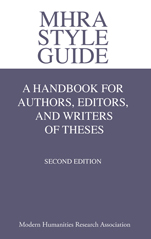
\includegraphics[scale=1.5]{hinh1}\\[1cm]
\end{flushleft}

\textbf{Tạo danh sách tham khảo và chú thích}.\\

Cho dù trích dẫn trực tiếp hoặc gián tiếp từ một nguồn,nguồn phải được công nhận
. Để tránh bị gián đoạn văn bản của bạn, chú thích, được đặt ở dưới cùng của trang, bao gồm thông tin tham khảo và được tách ra từ các văn bản chính. Trích dẫn có hình thức số thứ tự superscript (1, 2, 3 vv) được đặt sau khi một báo giá trực tiếp hoặc tham khảo một nguồn tin trong văn bản chính. Đây giới thiệu độc giả chú thích tương ứng ở dưới cùng của trang đó. Tất cả các nguồn được đề cập trong các trích dẫn phải được bao gồm trong danh sách các tài liệu tham khảo ở phần cuối của công việc của bạn. Bạn được yêu cầu phải cung cấp đầy đủ thông tin thư mục cho từng 
nguồn. Phải được liệt kê theo thứ tự chữ cái.\\

Các thành phần cơ bản để tham khảo mỗi thường bao gồm:

Tác giả (s) / Nhà xuất bản(s), Tiêu đề và chi tiết Xuất bản.
\\ {\bfseries Sách - hai hoặc nhiều tác giả}

Tham khảo danh sách / thư mục

Nolen, Stephanie và Jonathan Bate, khuôn mặt của Shakespeare (Melbourne: Văn bản Nhà xuất bản, 2002)

Đầu tiên chú thích

Stephanie Nolen và Jonathan Bate, Shakespeare Face (Melbourne: Văn bản Nhà xuất bản, 2002), trang 63-68.\\
{\bfseries Sách - thay đổi nội dung và sau đó ấn bản đầu tiên}\\
{\bfseries Sách - chương hoặc một bài báo làm việc hoặc trong cuốn sách thay đổi nội dung hoặc tuyển tập}

Tham khảo danh sách / thư mục

Stewart, JF Primitivism ở phụ nữ trong tình yêu ", đáp ứng quan trọng đối với DH Lawrence, chỉnh sửa bởi J. Pilditch (Westport, Conn: Greenwood Press, 2001)

Đầu tiên chú thích

JF Stewart, 'Primitivism ở phụ nữ trong tình yêu ", đáp ứng quan trọng để DH Lawrence, ed. J. Pilditch (Westport, CT: Greenwood Press, 2001), trang 246-59.

Tham khảo danh sách / thư mục

Johnson, Thomas H., ed, Emily Dickinson: Thư được chọn, xuất bản lần 2 (Cambridge, MA: Harvard University Press, 1985), trang 94, 105.

Đầu tiên chú thích

Emily Dickinson: chọn Letters, ed. Thomas H. Johnson, xuất bản lần 2 (Cambridge, MA: Harvard University Press, 1985), trang 94, 105.\\
{\bfseries Sách - thay đổi nội dung đa khối lượng tài liệu tham khảo làm việc như một từ điển bách khoa toàn thư}

Tham khảo danh sách / thư mục

Strayer, Joseph R., và những người khác, biên soạn, từ điển của thời Trung Cổ, 13 vols (New York: Scribner, 1982-1989), vi (1985)

Đầu tiên chú thích

Từ điển của thời Trung Cổ, ed. Joseph R. Strayer và những người khác, 13 vols (New York: Scribner, 1982-1989), vi (1985), 26.

{\bfseries Multi-khối lượng cuốn sách}

Tham khảo danh sách / thư mục

McKerrow, Ronald B., ed., Tác phẩm của Thomas Nashe, 2nd edn, rev. FP Wilson, 5 vols (Oxford: Blackwell, 1958)

Đầu tiên chú thích

Tác phẩm của Thomas Nashe, ed. Ronald B. McKerrow, 2nd edn, rev. FP Wilson, 5 vols (Oxford: Blackwell, 1958), iii, 94-98 (trang 95-96).



\subsection{The Elements of Style}
The Elements of Style (1918), còn được gọi là Strunk  White, bởi William Strunk, Jr. và EB White , là phong cách viết tiếng Anh một quy Mỹ hướng dẫn bao gồm tám "quy tắc cơ bản của việc sử dụng", mười nguyên tắc cơ bản của thành phần ", "một số vấn đề của hình thức", một danh sách 49 "từ và cụm từ thường được sử dụng sai mục đích", và một danh sách 57 "từ sai chính tả".
Năm 2011, tạp chí Time liệt kê các yếu tố của phong cách là một trong 100 cuốn sách tốt nhất và có ảnh hưởng nhất viết bằng tiếng Anh kể từ năm 1923.
\begin{flushleft}
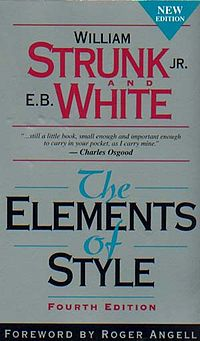
\includegraphics[scale=1]{hinh2}\\[1cm]
\end{flushleft}
\begin{flushleft}
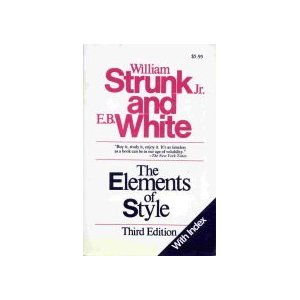
\includegraphics[scale=1]{hinh3}\\[1cm]
\end{flushleft}
Cover of 4th ed. (paperback, 2000)
Author(s)	William Strunk, Jr., and E.B. White\\
Country	USA\\
Language	English\\
Subject(s)	Style guide\\
Publisher	Pearson Education Company\\
Publication date	1919, 1959\\
Media type	Paperback book\\
Pages	105\\
ISBN	0-205-30902-X\\
OCLC Number	45802070\\
Dewey Decimal	808/.042 21\\
LC Classification	PE1408 .S772 1999\\


\subsection{The Elements of Typographic Style}
The Elements of Style Typographic là sách của dịch giả Robert Bringhurst . Xuất bản vào năm 1992 bởi nhà xuất bản Hartley và Marks , nó đã được sửa đổi vào năm 1996 , 2001 (v2.4), 2002 (v2.5), 2004 (v3.0), 2005 (v3.1), và 2008 (v3.2 ). Một lịch sử và hướng dẫn cho kiểu chữ , nó đã được ca ngợi bởi Hermann Zapf , người nói: "Tôi muốn nhìn thấy cuốn sách này trở thành chữ in Kinh Thánh."  Jonathan Hoefler và Tobias Frere-Jones xem xét nó "cuốn sách tốt nhất từng viết về kiểu chữ, "theo phần FAQ của trang web loại đúc. Bởi vì sử dụng rộng rãi của nó, nó đôi khi được viết tắt đơn giản là Bringhurst.

Ấn bản đầu tiên: Nhà xuất bản Hartley và Marks, năm 1993, 254pp, ISBN 0-88179-110-5 (bìa cứng).

Thứ hai phiên bản: Nhà xuất bản Hartley và Marks, năm 1996, 352pp, ISBN 0-88179-133-4 (bìa cứng), ISBN 0-88179-132-6 (bìa mềm)

Thứ ba phiên bản: Nhà xuất bản Hartley và Marks, 2005, ISBN 0-88179-205-5 (bìa cứng), ISBN 0-88179-206-3 (bìa mềm)\\


 Robert Bringhurst mang đến sự  rõ ràng cho nghệ thuật của kiểu chữ này hướng dẫn phong cách bậc thầy. Kết hợp thực tế, lý thuyết và lịch sử, phiên bản này là hoàn toàn cập nhật, với một thăm dò kỹ lưỡng của những cải tiến mới nhất trong công nghệ phông chữ thông minh, và phải có cho các nghệ sĩ đồ họa, biên tập viên, hoặc bất cứ ai làm việc với các trang in bằng cách sử dụng kỹ thuật số hoặc phương pháp truyền thống.


\subsection{ISO 690}
    ISO 690 là một ISO tiêu chuẩn cho thư mục tham khảo trong tài liệu của tất cả các loại  làm rõ cần bao gồm các tài liệu điện tử , và quy định cụ thể các yếu tố để được bao gồm trong các tài liệu tham khảo tài liệu xuất bản, và thứ tự mà các yếu tố của tài liệu tham khảo được công bố. Dấu chấm câu và phong cách không phải là một phần của tiêu chuẩn.\\

ISO 690 bao gồm tài liệu tham khảo đến các tài liệu được xuất bản trong cả in ấn và hình thức không in. Nó không áp dụng đối với tài liệu tham khảo bản thảo viết tay hoặc các vật liệu chưa được công bố khác [ cần dẫn nguồn ]. Phiên bản mới nhất đã được xuất bản vào năm 2010 và bao gồm tất cả các loại tài nguyên thông tin, bao gồm nhưng không giới hạn để chuyên khảo, serial, đóng góp, bằng sáng chế, vật liệu bản đồ, tài nguyên thông tin điện tử (bao gồm cả phần mềm máy tính và cơ sở dữ liệu), âm nhạc, ghi âm, bản in, hình ảnh , đồ họa và các tác phẩm nghe nhìn, và hình ảnh chuyển động.




ISO 690 là một tiêu chuẩn được phát triển bởi Ủy ban kỹ thuật ISO ISO / TC 46, Tiểu ban SC 9 của Tổ chức Quốc tế về Tiêu chuẩn hóa (ISO). Nó liên quan đến báo giá vật liệu của tất cả các loại và mô tả các yếu tố khác nhau để được bao gồm tài liệu tham khảo trong văn học và thứ tự của các yếu tố này.
ISO 690 bao gồm bất kỳ loại tài liệu xuất bản, dù là điện tử hay không. Tài liệu tham khảo cho các bản thảo viết tay hoặc bất kỳ tài liệu khác đã không được chủ đề của một ấn phẩm không được bảo hành theo tiêu chuẩn này.

\textbf{ Các bộ phận của tiêu chuẩn}

ISO 690 được mô tả trong hai tài liệu:\\
ISO 690:1987 (Tài liệu - tài liệu tham khảo thư mục - Nội dung, hình thức và cấu trúc) giao dịch với các tài liệu nói chung.\\
ISO 690-2:1997 (Thông tin và tài liệu hướng dẫn - thư mục tài liệu tham khảo - Phần 2: tài liệu điện tử, tài liệu hoặc các bộ phận của văn bản) đối phó với các tài liệu điện tử nói riêng.


\textbf{Đơn giản cuốn sách}\\
LOMINANDZE, DG Cyclotron sóng trong huyết tương. Dịch An. Dellis, thay đổi nội dung bởi SM. Hamberger. 1 ed. Oxford: Pergamon Press, 1981. 206 p. Loạt quốc tế trong triết học tự nhiên. Dịch: Ciklotronnye Volny v plazme. ISBN 0-08-021680-3.\\
\textbf{Thông qua một cuốn sách duy nhất}\\
PARKER, TJ. và Haswell, WD Text-cuốn sách về động vật học. Lần thứ 5, Vol. 1. Sửa đổi của WD. Lang. London: Macmillan, 1930. Mục 12, phylum Mollusca, p. 663-782.\\
\textbf{Đóng góp cho một cuốn sách duy nhất}\\
WRINGLEY, EA. Giáo xứ đăng ký và sử học. Trong thép, DJ quốc gia chỉ số của sổ đăng ký giáo xứ. London: Hội Genealogists, 1968, tập 1, trang 155-167.\\
\textbf{Nối tiếp}\\
Nhà sản xuất thiết bị thông tin liên lạc. Sản xuất năm Phòng Công nghiệp tiểu học, Thống kê Canada. Sơ bộ Edition, 1970 -. Ottawa: Thống kê Canada, 1971 -. Điều tra dân số hàng năm của nhà sản xuất. Văn bản bằng tiếng Anh và tiếng Pháp. ISSN 0700-0758.\\
\textbf{Điều trong một ấn phẩm định kỳ}\\
Weaver, William. Các nhà sưu tập: biểu diễn lệnh. Ảnh chụp bởi Robert Emmett Bright. Kiến trúc Digest, tháng 12 năm 1985, vol 42, số 12, trang 126-133.

\subsection{Phong cách trích dẫn APA }
{\bfseries Trích dẫn trong văn bản - tổng quan} \\
Khi viết theo cách suy nghĩ của bạn dự trên ý của một tài liệu tham khảo,bạn phải trích dẫn nguồn ban đầu\\
Vd:Ví dụ và giải thích thêm có sẵn trong phần 6 Chương 5 và Chương 7 của hướng dẫn sử dụng Xuất bản.\\
{\bfseries Phần tác giả:}\\
Một tác giả:\\hầu hết trường hợp cung cấp tên của tác giả và năm xuất bản là đủ.\\
Với 2 tác giả:\\Tên 2 tác giả và năm được công bố.\\
Vd: Như James và Ryerson (1999) đã chứng minh ... \\
Nếu có 3-5 tác giả:\\Trích dẫn tất cả các tác giả lần đầu tiên, trong các trích dẫn sau này, chỉ bao gồm tên cuối cùng của tác giả đầu tiên được theo sau bởi "et al." và các năm: \\
Vd:\\Williams, Jones, Smith, Bradner, và Torrington (1983) tìm thấy ... \\
Williams et al. (1983) cũng nhận thấy rằng ...\\
Nghiên cứu của một hiệp hội,một tổ chức:phải được nêu tên đầy đủ,tên viết tắt,và năm của báo cáo đó.Sau đó thì có thể viết tắt,chỉ sử dụng tên viết tắt,năm.\\Vd:(Viện Quốc gia Sức khỏe Tâm thần [NIMH], 1999) \\
{\bfseries Trích dẫn các phần cụ thể(trang,đoạn văn)}\\
Để trích dẫn một phần cụ thể của một nguồn, ta phải cho biết tác giả,năm,trang số mấy, chương trong nguồn.\\Vd:(Wilmarth, năm 1980, Chương 3).\\Đối với nguồn điện tử chẳng hạn như các trang Web, cung cấp một tham chiếu đến tác giả, năm và số trang (nếu nó là một tài liệu PDF).\\
{\bfseries Gián tiếp trích dẫn}\\
 Tên của tác giả ban đầu trong một câu giải thích, và sau đó bao gồm các nguồn mà bạn  tham khảo được đặt trong ngoặc đơn và trong danh sách tham khảo của bạn. \\Vd:Smith cho rằng ... (như trích dẫn trong Andrews, 2007)\\
{\bfseries Trích dẫn lời}\\Trích dẫn trực tiếp của nguồn\\Bạn có thể cho một tham chiếu trực tiếp đến nguồn để người đọc tự tham khảo,tìm hiểu.\\Trích dẫn đoạn ngắn :\\ Trích dẫn ít hơn 40 từ:văn bản được đặt trong ngoặc kép. Cung cấp các tác giả, năm xuất bản và số trang. \\VD: Miele (1993) found that "the 'placebo effect,' which had been verified in previous studies, disappeared when [only the first group's] behaviors were studied in this manner" (p. 276).\\Trích dẫn đoạn dài :\\Khi đưa ra một trích dẫn hơn 40 từ:sử dụng một "khối trích dẫn" tự do đứng trên một dòng,đoạn trích dẫn được thụt vào sâu hơn,và không có dấu ngoặc kép.\\
  {\bfseries Sách}\\  Cần nêu tên tác giả,năm xuất bản,tên tác phẩm,nơi xuất bản.\\
Vd:Bernstein, TM (1965) Hướng dẫn sử dụng tiếng anh. (2nd ed.). New York, NY: Atheneum.\\
Hai hay nhiều sách của một tác giả: trích dẫn theo thứ tự xuất bản.\\
Postman, N. (1979).Hoạt động bảo tồn. New York, NY: Delacorte Press.\\

Postman, N. (1985)Amusing ourselves to death: Public discourse in the age of show business . New York, NY: Viking.\\Sách của một hội đồng,tổ chức,cơ quan.\\Vd:Hiệp hội tâm lý Mỹ. (1972) tiêu chuẩn đạo đức của các nhà tâm lý học. Washington, DC: Hiệp hội tâm lý Mỹ.\\
{\bfseries Các bài viết}\\
     Bài viết trong một tờ báo hoặc tạp chí\\
Driedger, SD (năm 1998, ngày 20 tháng 4). Sau cuộc li hôn, 111 (16), 38-43.\\
Bài viết từ trang web : nêu tên tác giả,ngày lấy thông tin từ trang web,và địa chỉ trang web.\\
VdLandsberger, J. (n.d.). Chú thích trang web. Trong Hướng dẫn học tập. Rút ra vào ngày 13 tháng 5, 2005, từ http://www.studygs.net/citation.htm .\\
  {\bfseries Trích dẫn các tin đa phương tiện như truyền hình,video,radio.}\\
Truyền hình,chương trình phát thanh\\Vd: Bikel, Ofra. (Producer). 2009. Close to home [Television series episode]. \\
\subsection{MLA:}
 Có rất nhiều cách trích dẫn nguồn tài liệu tham khảo nhưng hiện nay, cách trích dẫn theo phong cách của MLA phổ biến nhất (MLA là chữ viết tắt của Modern Language Association – Hiệp hội Ngôn ngữ Hiện đại). Khi trích dẫn nguồn tài liệu, bạn cần lưu ý một số điểm chung như sau:
 

•	Tên sách hoặc tạp chí luôn phải gạch chân.

•	Nếu phần trích dẫn dài hơn 1 dòng thì dòng thứ hai phải lùi vào 5 ký tự.

•	Sắp xếp tên các tác giả trong bibliography theo thứ tự trong bảng chữ cái. Nếu không có tên tác giả thì căn cứ vào từ đầu tiên của tên bài để sắp xếp (không tính các quán từ “a”, “an”, “the”).

•	Nếu tác phẩm có nhiều hơn một tác giả thì liệt kê tên các tác giả theo thứ tự liệt kê trên trang bìa.

•	Nếu bạn chỉ sử dụng thông tin trong một bài của một cuốn sách hay một quyển tạp chí thì tên bài được trích dẫn trước tên sách, tên tạp chí.

•	 Phải tuân thủ cách trình bày (format) trong bibliography một cách chặt chẽ, kể cả từng dấu chấm, dấu phẩy. 


\subsubsection{Trích dẫn sách:}.

 Tên, họ tác giả. Tên sách. Thành phố: Nhà xuất bản, năm xuất bản.

•	Sách của một tác giả

Tên tác giả được liệt kê trước rồi mới đến họ. Tên sách được gạch chân. Sau đó liệt kê lần lượt tên thành phố, tên nhà xuất bản và năm xuất bản. Kết thúc trích dẫn phải có dấu chấm.

Ví dụ:

{\em Hingham, Cindy. Snowflakes for All Seasons. Salt Lake City: Gibbs Smith, 2004.}

•	Sách của hai tác giả

Tên của cả hai phải được trích dẫn và nối với nhau bằng từ “and”.

Ví dụ:

{\em Rhatigan, Joe and Newcomb, Rain. Prize Winning Science Fair Projects for Curious Kids.

New York: Lark Books, 2004.}

•	Sách có tên người biên tập

Thêm “ed” đằng sau tên người biên tập.

Ví dụ:

{\em Dickins, Rosie, ed. The Usborne Introduction to Art. Tulsa: EDC Publication, 2004.}

•	Sách không có tên tác giả

Trích dẫn tên sách đầu tiên.

Ví dụ:

{\em Fodor’s 05 Costa Rica. New York: Fodor’s Travel Publication, 2005.}

•	Trích dẫn một bài trong cuốn sách không có tên tác giả

Tên bài được trích dẫn trước tên sách và được đặt trong ngoặc kép cùng dấu chấm. Nếu tên thành phố xuất bản không quen thuộc với người đọc thì sẽ liệt kê thêm tên của bang hoặc đất nước.

Ví dụ:

{\em “Afghanistan.” Time Almanac. Needham, MA: Pearson Education Inc., 2005.}

\subsubsection{Trích dẫn từ điển bách khoa toàn thư và các loại sách tham khảo khác:}.	

Từ điển bách khoa toàn thư thường không có tác giả chung cho cả cuốn mà thường chỉ có tên của tác giả ở cuối mỗi bài trong từ điển.

•	 Những bài có tên trong từ điển bách khoa

Tên bài được đặt sau tên tác giả và phải đặt trong ngoặc kép.

Ví dụ:

Dunes, Alan. “Magic”. World Book Encyclopedia. Volume 13. Chicago: World Book Inc., 2005.

Những bài không có tên tác giả thì phần trích dẫn không có tên tác giả, các phần còn lại tương tự như những bài có tên tác giả.

\subsubsection{Trích dẫn tạp chí và báo:}.

•	Tạp chí có tên tác giả

Tên tác giả được đặt trước tên bài, sau đó là tên tạp chí, ngày xuất bản tạp chí, cuối cùng là số trang. Tên bài phải đặt trong ngoặc kép.

Ví dụ:

{\em Urbanas, Jason. “Bodies of Pompeii.” Dig. March 2005. Vol. 7: 16-17.}


•	Tài liệu tham khảo là bài báo

Tên tác giả. Tên bài báo được đặt trong ngoặc kép. Tên báo được gạch chân. Ngày tháng xuất bản. Mục, trang.

Ví dụ:

{\em FBI Agent “Risked Life” by Posing as Wise Guy.” Chicago Tribune. 10 March 2005. Section 1, Page 1}


\subsubsection{ Trích dẫn các trang web:}.

Nếu có tên tác giả thì đặt tên tác giả lên đầu tiên.Tên bài được gạch chân. Tiếp đến là ngày truy cập. Địa chỉ trang web được đặt trong ngoặc < >.
{\em Australian Scientists Prove Less Trees, Less Rain. 10 March 2005. <http://www.alertnet.org/thenews/newsdesk/syd269633.htm.>}
\subsection{Harvard:}.

Hệ thống trích dẫn theo tác giả-ngày tháng bắt nguồn từ đại học Harvard. Dù hiện nay trường Harvard không còn cung cấp một chỉ dẫn tham khảo chuẩn, các phiên

bản chỉ dẫn tham khảo theo kiểu tác giả-ngày tháng vẫn thường được gọi là phong

cách Harvard. Các phong cách chỉ dẫn tham khảo nổi tiếng khác có thể kể đến như
phong cách Chicago, APA (American Psychological Association) và MLA (Modern
Language Association).

Phong cách chỉ dẫn tài liệu tham khảo Harvard được công nhận rộng r.i trong giới học thuật. Mỗi chỉ dẫn tham khảo được viết bằng chữ gồm tác giả, ngày xuất bản, đôi khi đi kèm với các thông tin khác chẳng hạn như số trang.

\subsubsection{	Trích dẫn nguyên văn}.

Trong quá trình viết luận hay khóa luận cần chỉ dẫn tên tác giả và năm xuất bản của nguồn tài liệu tham khảo trong ngoặc đơn. Từ chỉ dẫn này, người đọc có thể t.m lạitheo trật tự bảng chữ cái nguồn đầy đủ của tài liệu chỉ dẫn trong phần danh mụctham khảo. Số trang là rất cần thiết khi tríc h dẫn nguyên văn từ một tác phẩm, sửdụng dấu ngoặc kép đi kèm số trang. Trong trường hợp tác phẩm trích dẫn có độ dàiđáng kể, số trang là vô cùng quan trọng để phục vụ cho người đọc t.m kiếm thôngtin thuận lợi hơn.

Ví dụ:


\subsubsection{Danh mục tài liệu tham khảo}.

Ở cuối tác phẩm, tác giả phải có danh mục tham khảo liệt kê TẤT CẢ những tài liệu tham khảo trong quá tr.nh viết. Theo phong cách trích dẫn Harvard, các nguồn tham khảo không được trích dẫn trực tiếp trong bài nhưng có liên quan đến chủ đề được liệt kê riêng trong phần Tài liệu tham khảo mở rộng. Phương pháp tr.nh bày sau được áp dụng cho cả danh mục Tài liệu tham khảo và Tài liệu tham khảo mở rộng.

Danh mục tham khảo được sắp xếp theo thứ tự bảng chữ cái đối với tên tác giả và
theo thứ tự thời gian xuất bản.

Ví dụ:

Hình thức chỉ dẫn tham khảo phụ thuộc vào loại tài liệu: sách, bài viết, website … Nói chung trật tự các thành phần trong một chỉ dẫn tham khảo phải bao gồm: tác giả - năm xuất bản – đầu đề/tên tác phẩm – tiêu đề tác phẩm – tiêu đề của tác
phẩm lớn hơn (nếu có) – nhà xuất bản – ngày xem/truy cập (nếu là điện tử). 


Trừ tên tác giả và ngày tháng, mỗi thông tin chi tiết trên phải cách nhau một dấu phẩy và kết thúc chỉ dẫn tham khảo bằng dấu chấm. 

\subsubsection{Tác giả}.

Bất cứ khi chỉ dẫn tham khảo một tài liệu nào, cách liệt kê tên tác giả phụ thuộc vào số tác giả của tài liệu.

\subsubsection{Sách}.

•	Toàn bộ sách

•	Hình thức:

Họ tác giả, Chữ cái viết tắt tên tác giả Năm xuất bản, Tên sách, Lần xuất bản, Nhà xuất bản, Nơi xuất bản.

Ví dụ:

Jones, B 1995, Sleepers, wake!: technology and the future of work , 4th edn, Oxford University Press, Melbourne.

•	Chương sách

•	H.nh thức:

Họ tác giả chương sách, Chữ cái viết tắt tên tác giả Năm xuất bản, Tiêu đề

chương’, [trong] Họ tac giả sách Chữ cái viết tắt tên tác giả sách (nếu khác với tác giả chương sách), Tên sách, Lần xuất bản, Nha xuất bản, Nơi xuất bản, Số trang.

Ví dụ:

{\em Crawford, RJ 1998, 'Plastics available to the designer', trong Plastics engineering, 3rd edn, Heinemann-Butterworth, Oxford, pp. 6-18.}

hoặc

{\em Christians, CG 2000, Ethics and poli tics in qualitative research, trong Denzin NK và Lincoln YS Handbook of qualitative research, 2nd edn, Thousand Oaks, CA, Sage, pp. 133-154.}

•	Sách điện tử từ Cơ sở dữ liệu điện tử

Nếu sách điện tử được lấy trên máy vi tính từ một cơ sở dữ liệu thư viện dưới dạng các file hình ảnh như Acrobat PDF, trích dẫn giống như sách in gốc. Nếu có nhiều hình thức trình duyệt sách điện tử khác nhau, nên lựa chọn định dạng file hình.

 Nếu sách điện tử từ dữ liệu thư viện được định dạng lại, chẳng hạn ở dạng HTML hoặc dạng plain text, hoặc từ một website, nên chỉ dẫn nguồn đa sử dụng vi những hình ảnh, biểu đồ, số trang… có thể bị mất đi. Nếu nguồn là từ một cơ sở dữ liệu thư viện, nếu tên cơ sở dữ liệu, hoặc nếu từ internet thi chỉ dẫn URL.
 
Hình thức:

Họ tác giả, Chữ viết tắt tên tác giả Năm xuất bản, Tên sách, Lần xuất bản, Nhà xuất bản, Nơi xuất bản, truy cập ngay tháng năm, tên cơ sở dữ liệu.

Ví dụ:

{\em Kung, SY, Mak, MW và Lin, SH 2004, Biometric authentication: a machine learning approach, Prentice Hall, Upper Saddle River, NJ., truy cập ngay 5 thang 8 năm 2005, Safari Tech Books Online.}

•	Sách điện tử từ Internet

Nếu sách điện tử thuộc cơ sở dữ liệu điện tử của thư viện dưới dạng cac file hinh như PDF, trích dẫn giống như sách in gốc. Nếu có nhiều hinh thức trình duyệt sách điện tử khác, nên chọn định dạng file hình. Nếu sách điện tử từ dữ liệu thư viện được định dạng lại, chẳng hạn ở dạng HTML hoặc dạng plain text, hoặc từ một website, nên chỉ dẫn nguồn đa sử dụng vi những hinh ảnh, biểu đồ, số trang… có thể bị mất đi. Nếu nguồn là từ cơ sở dữ liệu của thư viện, neu ten cơ sở dữ liệu, hoặc nếu từ internet thi chỉ dẫn URL.

Hình thức:

Họ tác giả, Chữ cái viết tắt tên tác giả Năm xuất bản, ‘Tên chương, [trong] sách của tác giả (nếu khác), Tên sách, Lần xuất bản, Nhà xuất bản, Nơi xuất bản, Truy cập ngày tháng năm, <URL>.

Ví dụ:

{\em Chen, C và Farruggia, S 2002, Culture and adolescent development, trong Lonner, WJ, Dinnel, DL, Hayes, SA và Sattler, DN (eds.), Online Readings in Psychology and Culture, Unit 11, Chapter 2, Center for Cross -Cultural Research, Western Washington University, Bellingham, Washington USA, viewed 15 September 2005, <http://www.ac.wwu.edu/culture/Chen Farruggia.htm>.}

•	Bách khoa toàn thư hoặc từ điển

Đối với nguồn từ bach khoa toan thư va từ điển, chỉ cần chỉ dẫn trong trường hợp trích dẫn nguyên văn trong bài, va KHÔNG cần đề cập tới trong Danh mục tham khảo.

Ví dụ:

{\em (Literacy in America: an encyclopedia 2001, p.25) khẳng định……}

•	Trích dẫn thứ cấp

Nguồn thông tin gốc rất quan trọng, tuy nhiên đôi khi không thể tìm ra nguồn thông tin gốc. Do đó buộc phải chỉ dẫn nguồn tham khảo từ trích dẫn của tác giả khác. Đây là nguồn thứ cấp, với trường hợp nay phải chỉ dẫn cả ten của tác giả va tên người trích dẫn đầu tiên khi trích dẫn nguyên văn. Danh mục tham khảo co thể chỉ cần liệt kê nguồn thứ cấp tìm thấy được.

Ví dụ trích dẫn nguyên văn:


{\em MacDonald (1993, trích dẫn trong Saunders, Lewis và Thornhill 2003, p. 48)} khẳng định

hoặc

{\em (MacDonald 1993, trích dẫn trong Saunders, Lewis  và Thornhill 2003, p. 48)}

Ví dụ danh mục tham khảo:

{\em Saunders, M, Lewis, P và Thornhill, A 2003, Research methods for business
students, 3rd edn, Pearson Educational, Essex, p. 48.}
•	Khuyết thời gian xuất bản

Các tác phẩm không có năm xuất bản sẽ dùng cụm viết tắt n.d. (no date) để biểu thị.

Ví dụ trích dẫn nguyên văn:

(Brown n.d.)

hoặc

Brown (n.d.)

Ví dụ danh mục tham khảo:

{\em Brown, S n.d. B. B. Bernard, Sunshine Press, London.}

\subsubsection{Bài viết chuyên ngành}.

Lưu ý: Viết hoa chữ cái đầu tiên của từ đầu tiên, và mỗi từ khóa trong tên bài viết.

Không in hoa các chữ như on, for, in, and


Vi dụ: The Australian Journal of Language and Literacy

Hình thức:

Tác giả của bai viết – Họ và chữ cái viết tắt tên tác giả Năm xuất bản, ‘Tên bài viết’, Tên tập san, số, kì phát hành, số trang.

Ví dụ:

{\em Zivkovic, B và Fujii, I 2001, An analysis of isothermal phase change of phase change material within rectangular and cylindrical containers, Solar Energy, số 70, kì phát hành 1, trang 51-61.}

•	Bài viết chuyên ngành điện tử từ CSDL

Lưu ý: Style manual for authors, editors and printers (2002) không phân biệt giữa nguồn tài liệu in hay điện tử. Chỉ dẫn tham khảo nguồn sach điện tử nên được thực hiện như sau. Nếu bài viết chuyên ngành thuộc cơ sở dữ liệu điện tử của thư viện dưới dạng các file hình như PDF, các bài viết này được trích dẫn tương tự như sách in gốc. Nếu có nhiều hình thức trình duyệt sách điện tử khác, nên chọn định dạng file hình. Nếu bài viết từ dữ liệu thư viện được định dạng lại, chẳng hạn ở dạng HTML hoặc dạng text trơn, hoặc từ một website, nen chỉ dẫn nguồn đa sử dụng vi những hinh ảnh, biểu đồ, số trang… có thể bị mất đi. Nếu nguồn là từ cơ sở dữ liệu của thư viện, nếu tên cơ sở dữ liệu, hoặc nếu từ internet thi chỉ dẫn URL.

Hình thức:

Tác giả của bài viết – Họ và chữ cái viết tắt tên tác giả Năm xuất bản, ‘Tên bài viết’, Tên tập san, số, số phát hành, số trang, truy cập ngày tháng năm, tên dữ liệu.

Ví dụ:

{\em Easthope, G 2004, 'Consuming health: the market for complementary and alternative medicine', Australian Journal of Primary Health , vol. 10, no. 2,  pp. 68- 75, viewed 30 March 2005, Australian Public Affairs Full Text.}

•	Bài viết có bản thảo được công bố trước khi được chỉnh l. và xuất bản (Inpress article)Hình thức:

Ten bai bao – Họ tác giả Chữ cái viết tắt tên tác giả có bản thảo được công bố, ‘Ten bai bao’, Tên tập san, xem ngày tháng năm, tên cơ sở dữ liệu (nếu có)

Ví dụ:

{\em Mundermann, A, Wakeling, JM, Nigg, BM, Humble, RN và Stefanyshyn, DJ in 14 press, Foot orthoses affect frequency components of muscle activity in the lowe lower extremity, Gait and posture, viewed 15 September 2005, ScienceDirect.}

\subsubsection{	Bài báo}.

Lưu ý: Viết hoa chữ cái đầu tiên của từ đầu tiên, và mỗi từ khóa trong tên bài báo.

Nếu bài báo khuyết danh thi chỉ cần chỉ dẫn cụ thể ở phần trich dẫn nguyên văn,
KHÔNG phải đưa vào Danh mục tham khảo.


Vi dụ: {\em The Australian (10 July 2002, p.1)} khẳng định……

Nội dung:

Họ tác giả, Chữ viết tắt ten tac giả Năm xuất bản, ‘Ten bai bao’, Tên tờ báo, ngay
thang, số trang.

Ví dụ:

{\em Tobler, K và Kerin, J 2002, Hormone alert for cancer, The Australian, 10 July, p.1.}

•	Bài báo từ cơ sở dữ liệu

Nếu bài báo thuộc cơ sở dữ liệu điện tử của thư viện dưới dạng cac file hinh ảnh như PDF, các bài báo này được trích dẫn giống như sách in gốc. Nếu có nhiều hình thức trình duyệt sách điện tử khác, nên chọn định dạng file hinh. Nếu bai bao từ dữ liệu thư viện được định dạng lại, chẳng hạn ở dạng HTML hoặc văn bản thuần tuý, hoặc từ một website, nên chỉ dẫn nguồn đa sử dụng vi những hình ảnh, biểu đồ, số trang… có thể bị mất đi. Nếu nguồn là từ cơ sở dữ liệu của thư viện, nếu tên cơ sở dữ liệu, hoặc nếu từ internet thì chỉ dẫn URL.

Hình thức:

Họ tác giả, Chữ cái viết tắt tên tác giả Năm xuất bản, ‘Tiêu đề bài báo’, Tên báo, ngày tháng, số trang, xem ngày tháng năm, tên dữ liệu cơ sở.

Ví dụ:

{\em Timmins, N 2005, ‘Delay raises doubt in public sector’, Financial Times, 20 July, truy cập 21 July 2005, Factiva.}

•	Bài đăng trên diễn đàn thảo luận (Discussion List Message)

Hình thức:

Tác giả <địa chỉ hòm thư điện tử của tác giả> Năm đăng bài, ‘Tên bài đăng, mo tả bài đăng, ngày và tháng đăng bài, tên chủ diễn đàn, truy cập ngày tháng năm, <URL>.

Ví dụ:

{\em Shively, E <chminf-l@listserv.indiana.edu> 1997, ‘CA pre -1967 information’, list server, 1 July, Chemical Information Sources Discussion List, viewed 3 July 2003,}

{\em <http://listserv.indiana.edu/archives/chminf -l.html>.}


•	Bài đăng trên diễn đàn thông tin (Newsgroup message)

Hình thức:


Tác giả <địa chỉ hòm thư điện tử của tác giả> Năm đăng bai, ‘Ten bai đăng’, mô tả bài đăng, ngày và tháng đăng bài, Tên chủ diễn đàn, truy cập ngay tháng năm, <URL>.

Ví dụ:

{\em Milinkovich, M 2005, ‘Oracle PL/SQL in Eclipse’, diễn đan, 12 July, News.Eclipse.Technology, 15 September 2005,

<http://dev.eclipse.org/newslists/news.eclipse.technology/msg01045.html>,
}
•	Bài đăng trên Blogs

Hình thức:

Tác giả <địa chỉ hòm thư của tác giả> Năm đăng bài, ‘Tên bài đăng’, mô tả bài đăng, ngày và tháng đăng, Tên nhà cung cấp blog, ngày tháng truy năm truy cập, <URL>.

Ví dụ:

{\em Steffen, A 2005, ‘Bird flu can we out -collaborate a pandemic?’ blog, 15 August, World Changing: another world is here , viewed 15 September 2005, <http://www.worldchanging.com/archives/003310.html>.}

•	Các tài liệu từ website

Rất nhiều nguồn tài liệu điện tử không đánh số trang trừ cac tài liệu ở dạng PDF. Nếu trích dẫn hoặc diễn giải từ một website ma tai liệu không ở dạng PDF, vẫn có thể sử dụng làm một phần của trích dẫn nguyên văn trong bài.

• đề mục, (eg. Stone 2004, Usage and prognosis section)

• số đoạn (eg. Stone 2004, para.11)

H.nh thức:

Tác giả/Biên tập viên. Năm xuất bản, Tên tài liệu, tên người bảo trợ nguồn, ngày truy cập, <URL>.

Ví dụ danh mục tham khảo:

{\em Stone, A 2004, Headaches due to Wind Cold, Al Stone Acupuncture and Traditional Chinese Herbal Medicines, truy cập 10 September 2006,  <http://beyondwellbeing.com/headaches/wind -cold.shtml >.}


\subsubsection{	Những nguồn khác}.

•	Kỷ yếu hội thảo

Hình thức:

Họ tác giả, Chữ viết tắt tên tác giả Năm xuất bản, ‘Tiêu đề biên bản’, [trong] Biên tập viên (nếu có), Tên kỷ yếu được xuất bản có thể gồm địa điểm và thời gian tổ chức, Nhà xuất bản, Nơi xuất bản, số trang.


Ví dụ:

{\em Kovacs, GL 1994, ‘Simulation-scheduling system using hybrid software}

{\em 17 technology’, trong Computer Integrated Manufacturing and Automation

Technology: Proceedings of the 4th International conference, Troy, New York, October 10-12, 1994, IEEE Computer Society Press, Los Alamitos, California, pp.351-356.}

•	Khóa luận/ Luận văn

•	Bằng sáng chế

Hình thức:

Tên nhà phát minh. Tên người được ủy quyền, Tên sáng chế, Số sáng chế Thời điểm sáng chế (gồm ngày và tháng).

Ví dụ:

{\em Wilmott, JM và Znaiden, AP Avon Products Inc., Cosmetic preparation

incorporating stabilized ascorbic acid , U.S. patent 4,983,382 Jan. 8 1991.}

•	CD ROM

Hình thức:

Tên tác giả/biên tập viên, Chữ viết tắt tên tác giả/biên tập viên Năm, Tiêu đề, Lần xuất bản, CD-ROM, Nhà xuất bản, Nơi xuất bản.
Ví dụ:


{\em Young, B và Heath, J 2000, Wheater's functional histology : a text an d colour atlas, 4th edn, CD-ROM, Churchill Livingstone, Edinburgh.}

•	Phim, video, chương tr.nh truyền h.nh và chương trình radio

Hình thức:

Tên chương trình Ngày thu, hình thức, nhà xuất bản, địa điểm thu, thời điểm xem.

Ví dụ:

{\em What are we going to do with the money? 1997, television program, SBS Television, Sydney, 8 August.}

Hoặc

{\em Swiss ball: exercises for performance and function 1999, video recording, Galaxy Leisure Corporation, 3 February.}\begin{scriptsize}
•
\end{scriptsize}

\section{So sánh giữa các chuẩn  }\label{result}
Nhìn chung các chuẩn không khác nhau trong cách trình bày trong latex.\\
{\bfseries Nhưng các chuẩn đều phải thỏa các quy tắc sau đây:}\\
  Dẫn liệu của một tác giả 
 cách viết này áp dụng cho cách viết của đồng tác giả hay nhiều tác giả\\
* Theo Nair(1987), kỹ thuật canh tác theo băng có thể giữ vai trò quan trọng ...\\....


Lưu ý: các dấu vòng đơn () đặt sát năm công bố và cách một ký tự rỗng với từ phái trước, dấu phẩy()<sát với cụm từ phía trước .\\
Dẫn liệu của đồng tác giả
thì phải liệt kê đủ hai kết quả.


%%%%%%%%%%%%%%
\section{Kết Luận }\label{result}
Tham khảo và trích dẫn tài liệu trong quá trình nghiên cứu là không thể tránh khỏi. Việc trính dẫn tài liệu và nguồn tham khảo vừa làm cho tài liệu thêm chính xác, tăng sức thuyết phục, thể hiện trình độ của người viết , mà việc trích dẫn nguồn thể hiện thái độ tôn trọng với tác giả, tạo cơ sở chắc chắn đối với người tham khảo\\\.
Trên đây chúng tôi đã liệt kê những chuẩn khai báo tài liệu trích dẫn khá phổ biến hiện nay, mỗi cách có các đặc điểm riêng, có những điểm mạnh và nhược điểm riêng, mỗi người cần lựa chọn cách trích dẫn phù hợp , để vừa dễ sử dụng và hiệu quả. \\
Tài liệu được thực hiện  với sự giúp đỡ tận tình của giáo viên hướng dẫn cùng sự cố gắng của các thành viên trong nhóm.\\
Trong quá trình nghiên cứu, thực hiện không thể tránh khỏi những  thiếu sót, kính mong quý thầy  cô và các bạn đóng góp thêm để tài liệu thêm hoàn thiện.\\
Xin chân thành cảm ơn.




%%%%%%%%%%%%%%
\section{Tài liệu Tham Khảo }




%%%%%%%%%%%%%%%%%%%%%%%%%%%%%%%%%

Tham  khảo chủ yếu từ web: http://en.wikipedia.org\\
http://globaledu.com.vn/Thong-Tin-Chi-Tiet/1881/1881\\
http://library.williams.edu/citing/styles/acs.php\\

%%%%%%%%%%%%%%
\newpage
\section{Phân công công việc}\label{conclusion}
Huỳnh Tấn Ngàn -MSSV: 51102184: Mục 3.1, 3.2, 3.3, 3.4.
\\Nguyễn Quốc Long-MSSV: Mục  3.6, 3.7, 3.8, 3.9.
\\Đinh Tấn Lộc-MSSV:51101935: 3.10, 3.11.
\\Nguyễn Sang Trường Sơn -MSSV:51102938: Mục 3.12 và 3.5
\\Các mục còn lại như giới thiệu, kết luận và phần so sánh sự khác nhau của các chuẩn được cả nhóm thảo luận và làm chung.
\end{document}



